\documentclass[tikz,border=2pt]{standalone}
\usepackage{amsmath}
\usepackage{amssymb}
\usepackage{pgfplots}
\pgfplotsset{compat=1.18}
\usetikzlibrary{arrows.meta}
\begin{document}
% Load with setups: rho(B) = lambda E[S] = lambda (E[S_0] + E[R]/B) = 0.75 + 6/B for lambda = 3/h,
% E[S_0] = 1/4 h, E[R] = 2 h; rho = 1 at B_m = 24, rho(20) = 1.05, rho(25) = 0.99, rho(30) = 0.95.
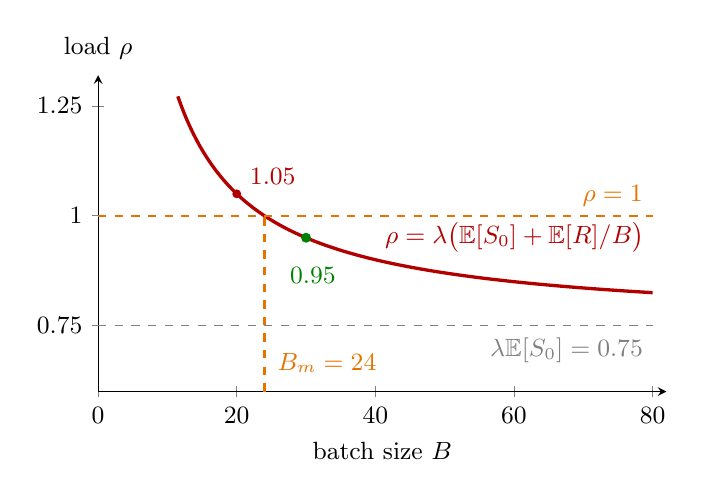
\begin{tikzpicture}[font=\small, >={Latex[length=2mm]}]
  \begin{axis}[
    axis lines=left, xmin=0, xmax=82, ymin=0.6, ymax=1.32,
    xtick={0,20,40,60,80},
    ytick={0.75,1,1.25},
    xlabel={batch size $B$}, ylabel={load $\rho$},
    ylabel style={rotate=-90, anchor=south, at={(axis description cs:0,1.02)}},
    samples=150, width=8.8cm, height=5.6cm, clip=false]
    \addplot[red!70!black, very thick, domain=11.5:80] {0.75+6/x};
    \draw[gray, thin, dashed] (axis cs:0,0.75) -- (axis cs:80,0.75);
    \node[gray, anchor=north east] at (axis cs:80,0.745) {$\lambda\mathbb{E}[S_0]=0.75$};
    \draw[orange!90!black, thick, dashed] (axis cs:0,1) -- (axis cs:80,1);
    \draw[orange!90!black, thick, dashed] (axis cs:24,0.6) -- (axis cs:24,1);
    \node[orange!90!black, anchor=south west] at (axis cs:24.5,0.62) {$B_m=24$};
    \node[orange!90!black, anchor=south east] at (axis cs:80,1) {$\rho=1$};
    \fill[red!70!black] (axis cs:20,1.05) circle (1.6pt);
    \node[red!70!black, anchor=south west] at (axis cs:20.5,1.05) {$1.05$};
    \fill[green!50!black] (axis cs:30,0.95) circle (1.8pt);
    \node[green!50!black, anchor=north] at (axis cs:31,0.905) {$0.95$};
    \node[red!70!black, anchor=west] at (axis cs:40,0.95) {$\rho=\lambda\bigl(\mathbb{E}[S_0]+\mathbb{E}[R]/B\bigr)$};
  \end{axis}
\end{tikzpicture}
\end{document}
